\chapter{Desenvolvimento}

\section{Definição do Produto e Fluido Refrigerante}

Para o desenvolvimento do projeto, definiu-se como produto a ser refrigerado o pescado fresco, recebido na câmara frigorífica a \textit{0°C} e armazenado em temperatura de conservação de \textit{-25°C}, condição típica para armazenamento comercial de longo prazo. As propriedades termofísicas do produto, incluindo calor específico, densidade e calor latente de congelamento, bem como as temperaturas de operação, encontram-se especificadas na Tabela~\ref{massa peixe}.

A seleção do fluido refrigerante considerou critérios técnicos, econômicos e ambientais. O refrigerante R-134a (1,1,1,2-tetrafluoretano) foi escolhido por apresentar características adequadas à faixa de temperatura requerida, baixo custo relativo, ampla disponibilidade no mercado e extensa utilização em aplicações de refrigeração comercial. Adicionalmente, o R-134a possui potencial de destruição da camada de ozônio (ODP) nulo, embora apresente potencial de aquecimento global (GWP) moderado de 1430, sendo considerado um fluido de transição aceitável para esta aplicação.

As propriedades termodinâmicas do R-134a, incluindo entalpia, entropia, temperatura e pressão em diferentes estados do ciclo, foram determinadas através da biblioteca CoolProp, uma base de dados de código aberto amplamente validada. A integração com rotinas computacionais desenvolvidas em Python permitiu o cálculo automatizado dos ciclos de refrigeração e a análise paramétrica do sistema.

\section{Estimativa da Carga Térmica de Refrigeração}

A seleção adequada do compressor requer inicialmente a determinação da carga térmica do sistema, que corresponde à taxa de calor a ser removida do produto durante o processo de resfriamento. Para este projeto, considerou-se uma câmara frigorífica com capacidade volumétrica de 200 litros, operando com fator de ocupação de 70\%, o que resulta em uma massa de pescado de aproximadamente 136 kg, conforme a Equação~\ref{massa peixe}.

\begin{equation}
    m_{\text{peixe}} = \rho \cdot V_{\text{útil}}
    \label{massa peixe}
\end{equation}

O tempo de \textit{pull-down}, isto é, o período necessário para reduzir a temperatura do produto desde a condição inicial (0°C) até a temperatura de armazenamento (-25°C), foi especificado em 8 horas. Este parâmetro é crítico para o dimensionamento, pois define a potência mínima de refrigeração necessária. A carga térmica sensível foi calculada pela Equação~\ref{Q resfriamento}, considerando apenas a remoção de calor sensível do pescado, sem contemplar a fase de congelamento.

\begin{equation}
    \dot{Q}_{\text{produto}} = \frac{m \cdot c \cdot \Delta T}{\Delta t}
    \label{Q resfriamento}
\end{equation}

\begin{table}[ht]
\centering
\begin{tabular}{|l|c|c|}
\hline
\textbf{Parâmetro} & \textbf{Símbolo} & \textbf{Valor} \\ \hline
Densidade do pescado & $\rho$ & 972 kg/m³ \\ \hline
Volume útil da câmara & $V_{\text{útil}}$ & 0,14 m³ \\ \hline
Calor específico do pescado & $c$ & 1,71 kJ/(kg·K) \\ \hline
Variação de temperatura & $\Delta T$ & 25 K \\ \hline
Tempo de \textit{pull-down} & $\Delta t$ & $2,88 \times 10^{4}$ s (8 h) \\ \hline
\end{tabular}
\caption{Parâmetros utilizados no cálculo da carga térmica do produto.}
\label{tab:tabela dados}
\end{table}

Substituindo os valores da Tabela~\ref{tab:tabela dados} na Equação~\ref{Q resfriamento}, obtém-se a carga térmica mínima requerida:

\begin{equation}
    \dot{Q}_{\text{produto}} = 202,6~\text{W}
    \label{carga}
\end{equation}

É importante ressaltar que este valor representa apenas a carga térmica do produto. Em um projeto completo, deveriam ser consideradas cargas térmicas adicionais, como infiltração de ar, ganho de calor pelas paredes, iluminação e respiração do produto, que podem aumentar significativamente a carga total do sistema.

\subsection{Seleção de Compressores Candidatos}

Com a carga térmica de referência estabelecida, procedeu-se à seleção de compressores candidatos através da ferramenta \textit{Product Selector} disponibilizada pelo fabricante Embraco. Para aplicações em baixas temperaturas de evaporação, como a especificada neste projeto (-25°C), são recomendados compressores da linha LBP (\textit{Low Back Pressure}), projetados especificamente para trabalhar com elevadas razões de compressão.

\begin{figure}[ht]
    \centering
    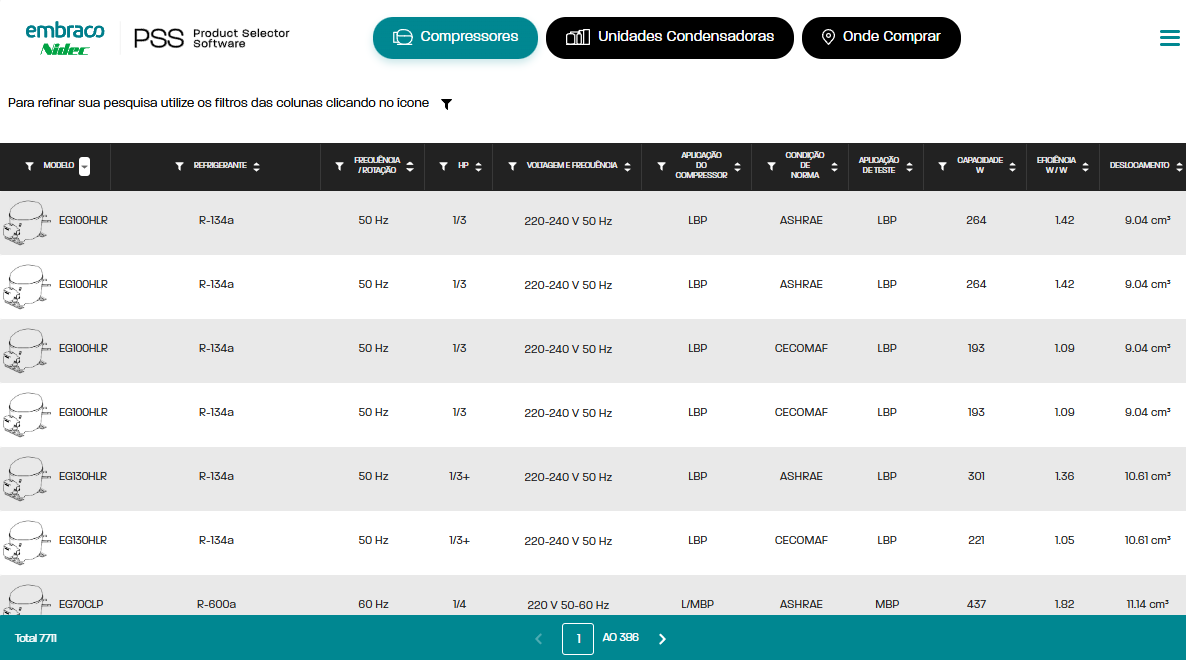
\includegraphics[width=0.8\linewidth]{Imagens/Desenvolvimento/PSS-embraco.png}
    \caption{Interface do seletor de produtos Embraco utilizado para pré-seleção dos compressores.}
    \label{fig:seletor de produtos}
\end{figure}

Os catálogos técnicos dos compressores pré-selecionados fornecem dados de desempenho obtidos em condições padronizadas de teste, incluindo temperaturas de evaporação e condensação, capacidade de refrigeração, consumo de potência elétrica e corrente nominal. Estes dados permitem uma análise comparativa detalhada do desempenho termodinâmico e econômico de cada modelo.

Foram selecionados quatro modelos de compressores herméticos que atendem aos requisitos de capacidade de refrigeração, apresentados na Tabela~\ref{tab:compressores escolhidos}.

\begin{table}[ht]
\centering
\begin{tabular}{|l|c|c|}
\hline
\textbf{Modelo} & \textbf{Potência Nominal [W]} & \textbf{Custo Estimado [R\$]} \\ \hline
EGAS80HLR & 240 & 650 \\ \hline
EGZS60HLP & 180 & 1340 \\ \hline
EGZS70HLC & 202 & 1130 \\ \hline
FFU70HAK & 221 & 600 \\ \hline
\end{tabular}
\caption{Compressores pré-selecionados para análise comparativa.}
\label{tab:compressores escolhidos}
\end{table}

\newpage

\section{Ciclo de Refrigeração Padrão:}

Com os dados preliminares obtidos, foi desenvolvida uma rotina em Python para calcular as propriedades do sistema, de acordo com o ciclo descrito na Figura \ref{fig:ciclo padrão}. 

\begin{figure}[ht]
    \centering
    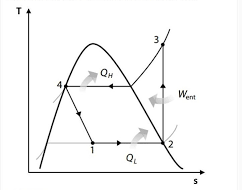
\includegraphics[width=0.6\linewidth]{Imagens/Desenvolvimento/Diagrama.png}
    \caption{Ciclo padrão.}
    \label{fig:ciclo padrão}
\end{figure}

\newpage

O programa utiliza um método iterativo para determinar a  mínima temperatura operacional possível, com o objetivo de reduzir custos ao evitar o superdimensionamento do compressor, utilizando como base os parâmetros descritos a seguir:

\begin{equation}
    \dot{Q_L} = \dot{m}(h_1-h_4)
    \label{QL}
\end{equation}

\begin{equation}
    \dot{Q_H} = \dot{m}(h_2-h_3)
    \label{QH}
\end{equation}

    Onde $\dot{Q_L}$ e $\dot{Q_H}$, são  a taxa com que sai e que entra calor no sistema, respectivamente. O trabalho do compressor pode ser calculado apartir da equação \ref{W compressor}, utilizando as propriedades do fluido antes e depois da compresão.

\begin{equation}
    \dot{W_{comp}} = \dot{m}(h_2-h_1)
    \label{W compressor}
\end{equation}

\begin{equation}
    \Delta h_{1-2} \simeq  c_p (T_2-T_1)
    \label{simplificacao entalpia}
\end{equation}

    E a eficiência do sistema é dada como:

\begin{equation}
    COP = \frac{T_H}{T_H - T_L}
    \label{COP carnot}
\end{equation}

\newpage    

Simultaneamente, são calculadas as propriedades do fluido refrigerante em cada estado do ciclo de refrigeração. Para efeito de comparação com o ciclo real, também é realizado o cálculo do ciclo ideal de Carnot, a fim de se obter a eficiência máxima possível e as temperaturas mínimas requeridas pelo sistema.

Depois de uma rodada de anállises, dois compressores destacaram-se, o desempenho de ambos nos ciclos pode ser visto nas figuras \ref{fig:ciclo comp 1} e \ref{fig:ciclo comp 2}.

\begin{figure}[ht]
    \centering
    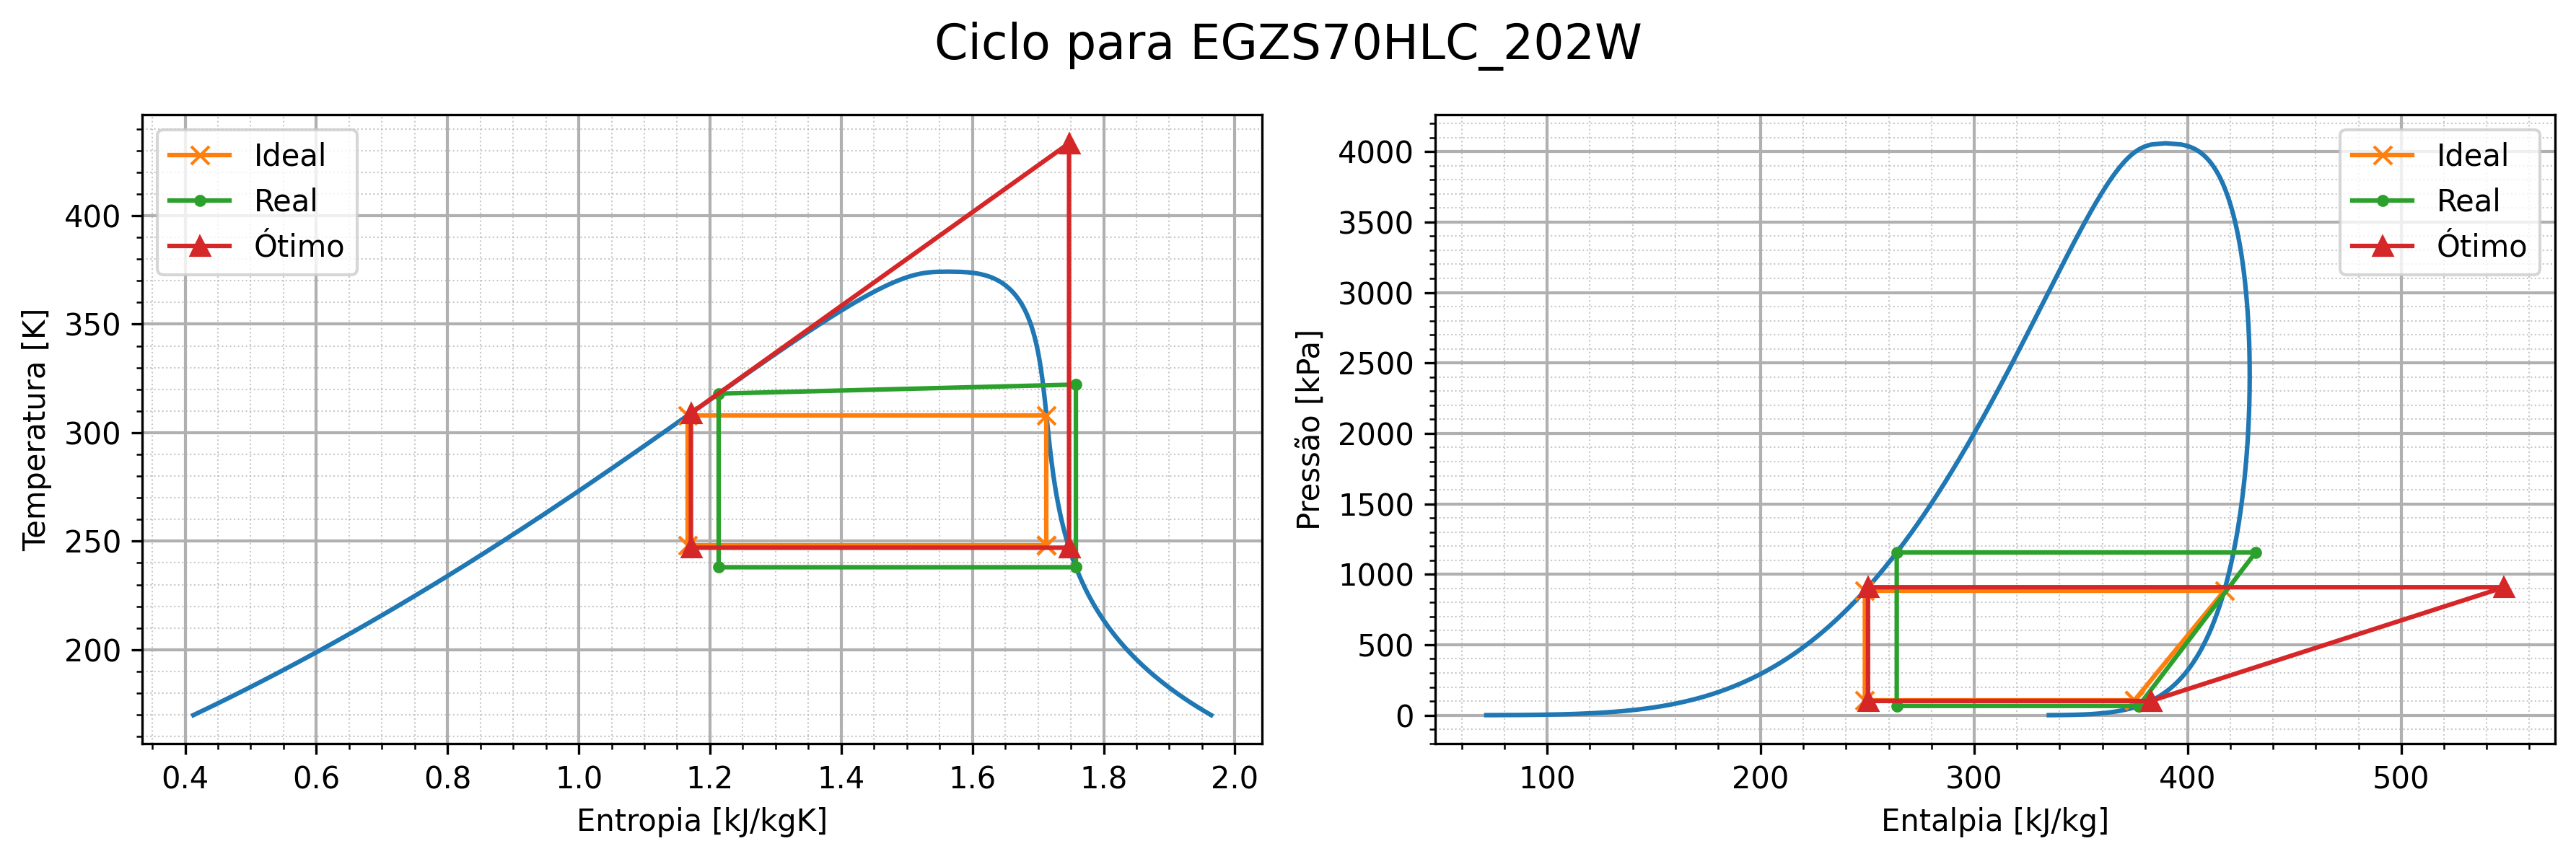
\includegraphics[width=0.9\linewidth]{Imagens/Desenvolvimento/ciclo_EGZS70HLC_202W.png}
    \caption{Ciclo para o EGZS70HLC.}
    \label{fig:ciclo comp 1}
\end{figure}

\begin{figure}[ht]
    \centering
    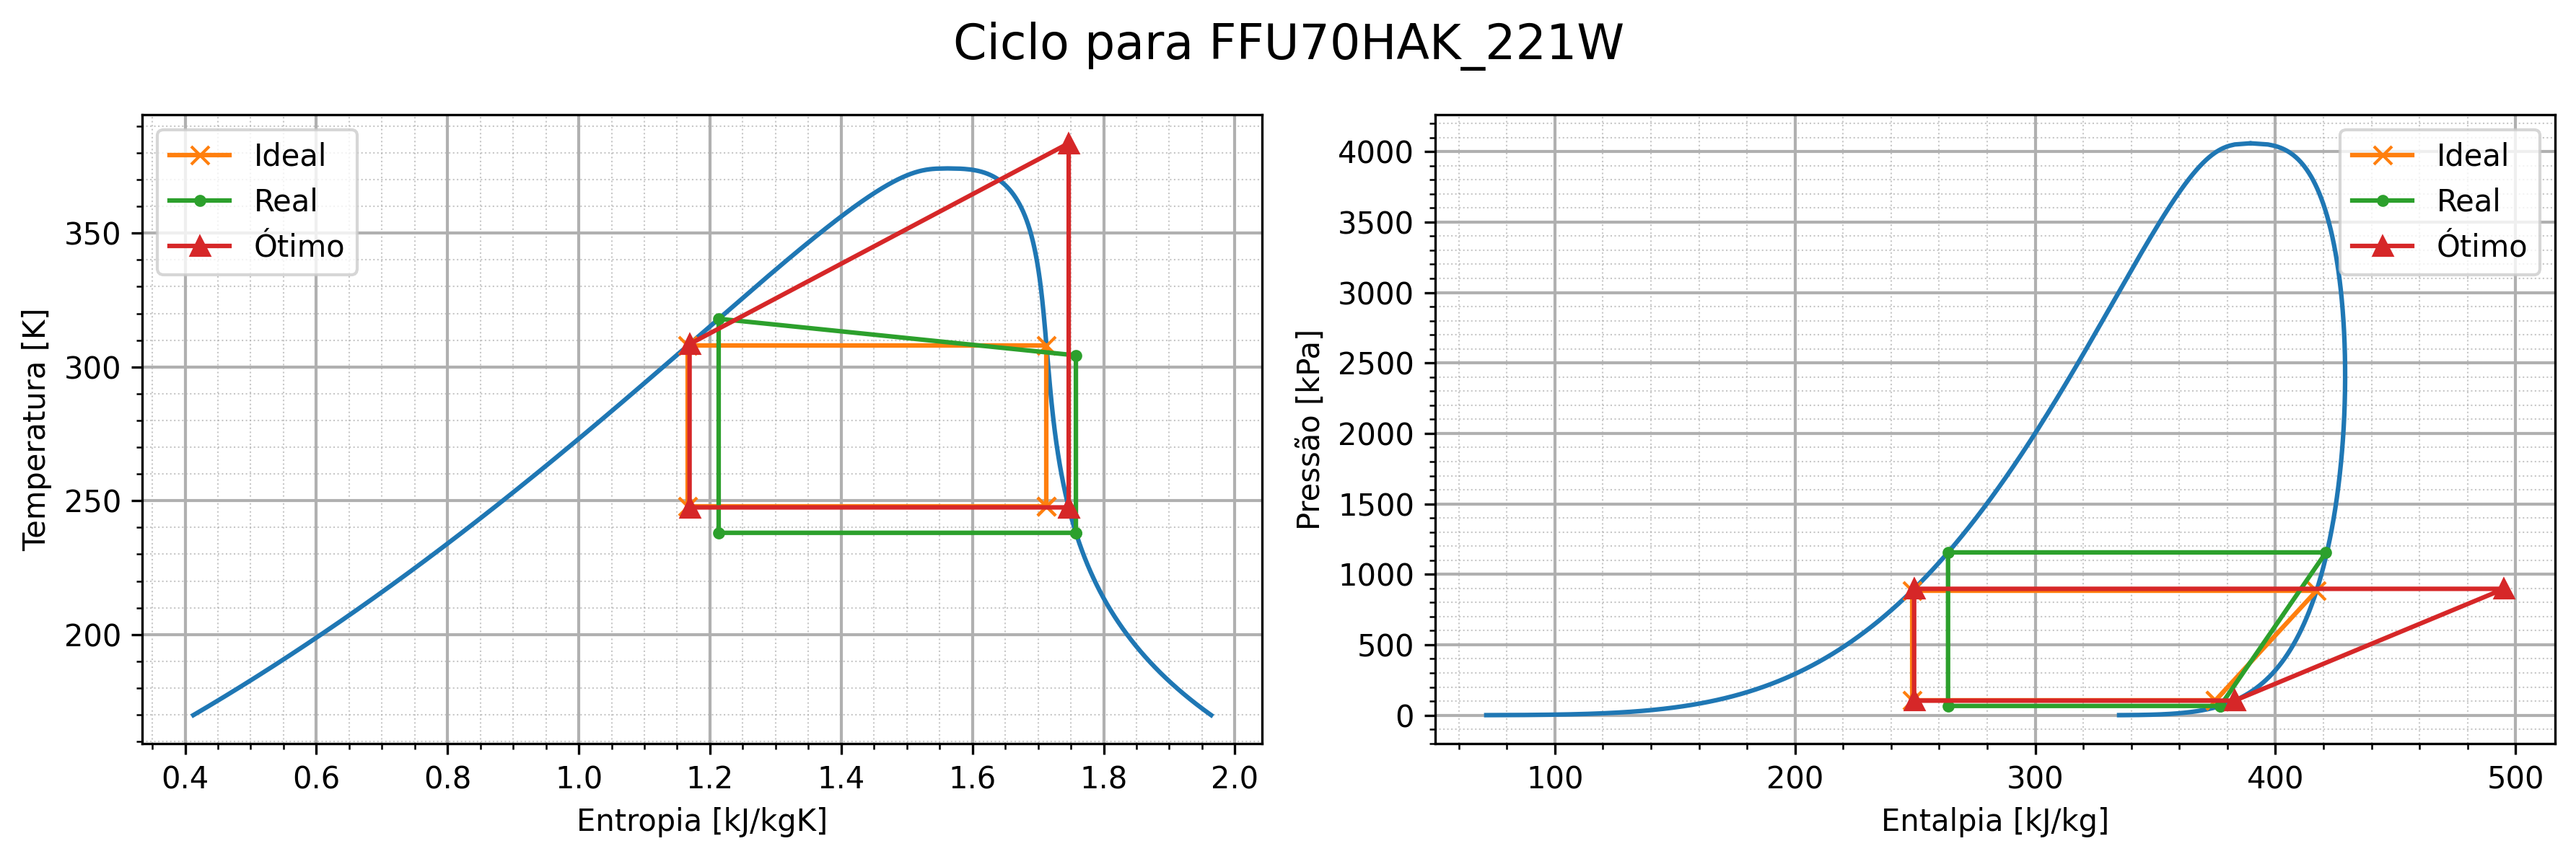
\includegraphics[width=0.9\linewidth]{Imagens/Desenvolvimento/ciclo_FFU70HAK_221W.png}
    \caption{Ciclo para o FFU70HAK.}
    \label{fig:ciclo comp 2}
\end{figure}

É possivél notar uma grande diferença entre o ciclo real e o ótimo, causada pelas perdar do sistema real, que aparecem em forma de calor. A rotina desenvolvida também calcula outros parâmetros de desempenho do sistema, tais como fluxo mássico, potência, COP e ${Q_L}$.

\newpage

\begin{figure}[ht]
    \centering
    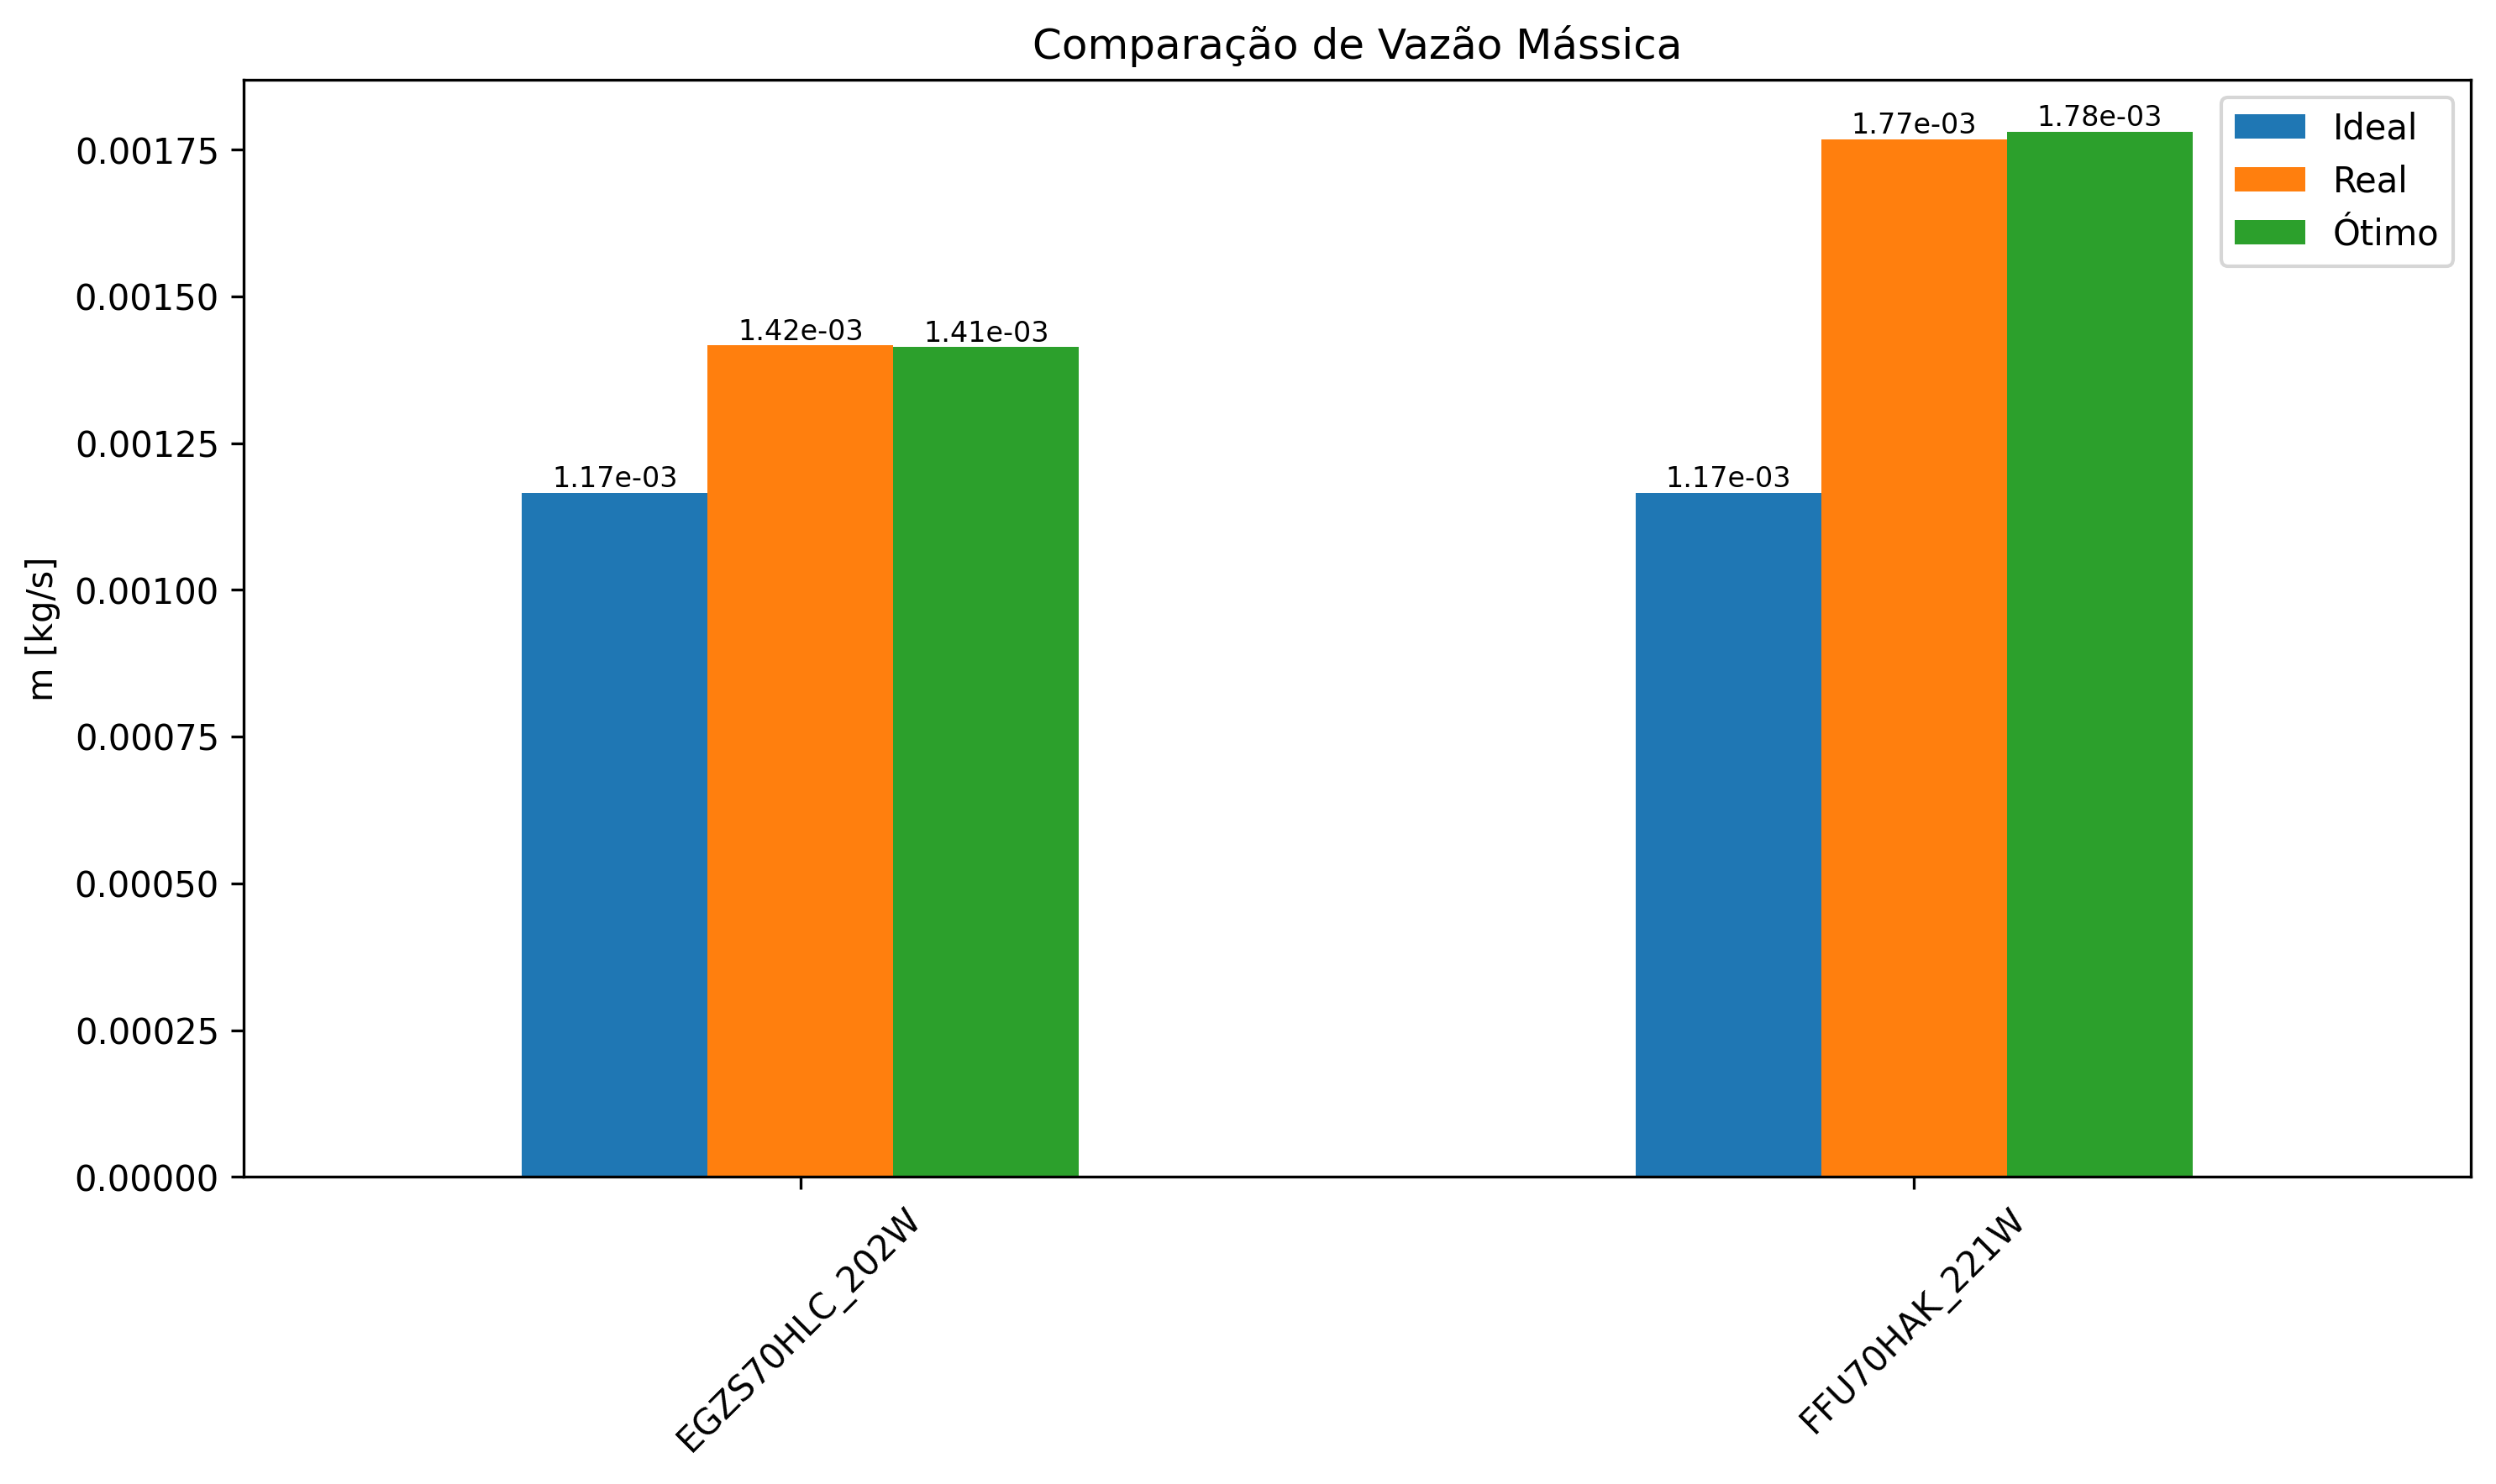
\includegraphics[width=0.8\linewidth]{Imagens/Desenvolvimento/barras_m.png}
    \caption{Compração do $\dot{m}$.}
    \label{fig:barras fluxo massa}
\end{figure}

\begin{figure}[ht]
    \centering
    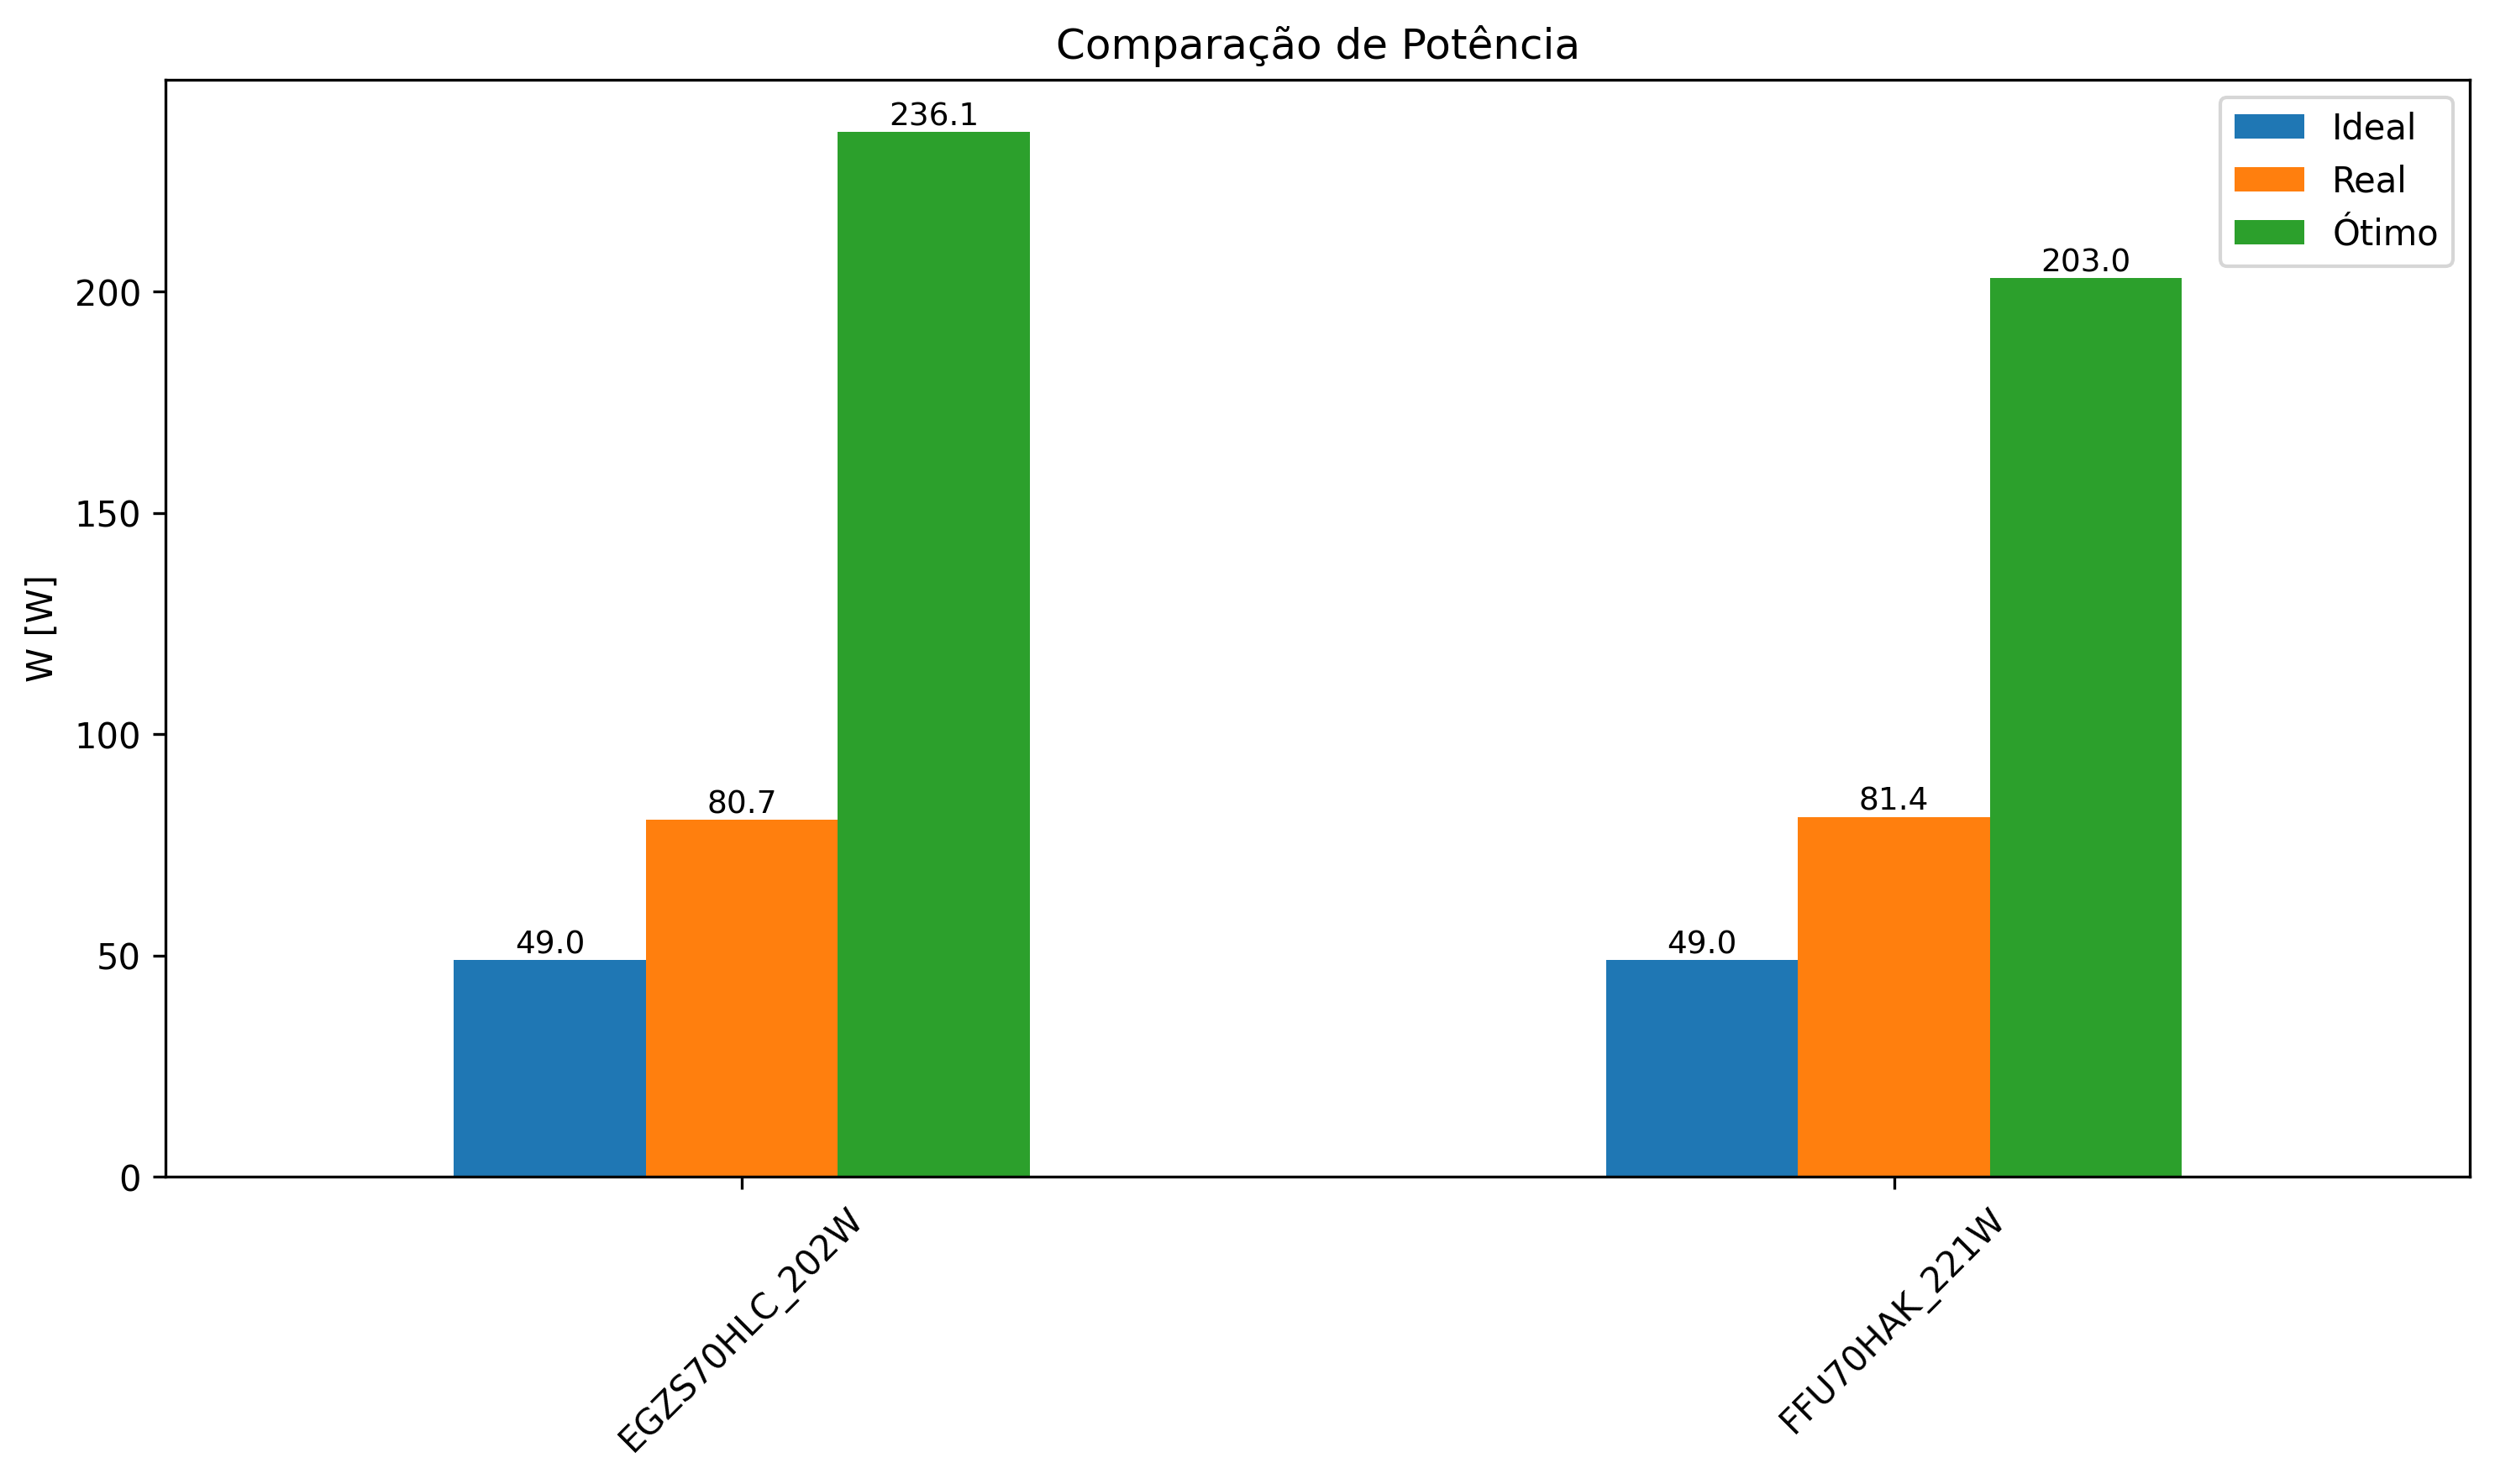
\includegraphics[width=0.8\linewidth]{Imagens/Desenvolvimento/barras_W.png}
    \caption{Compração da potência.}
    \label{fig:barras W}
\end{figure}

\newpage

\begin{figure}[ht]
    \centering
    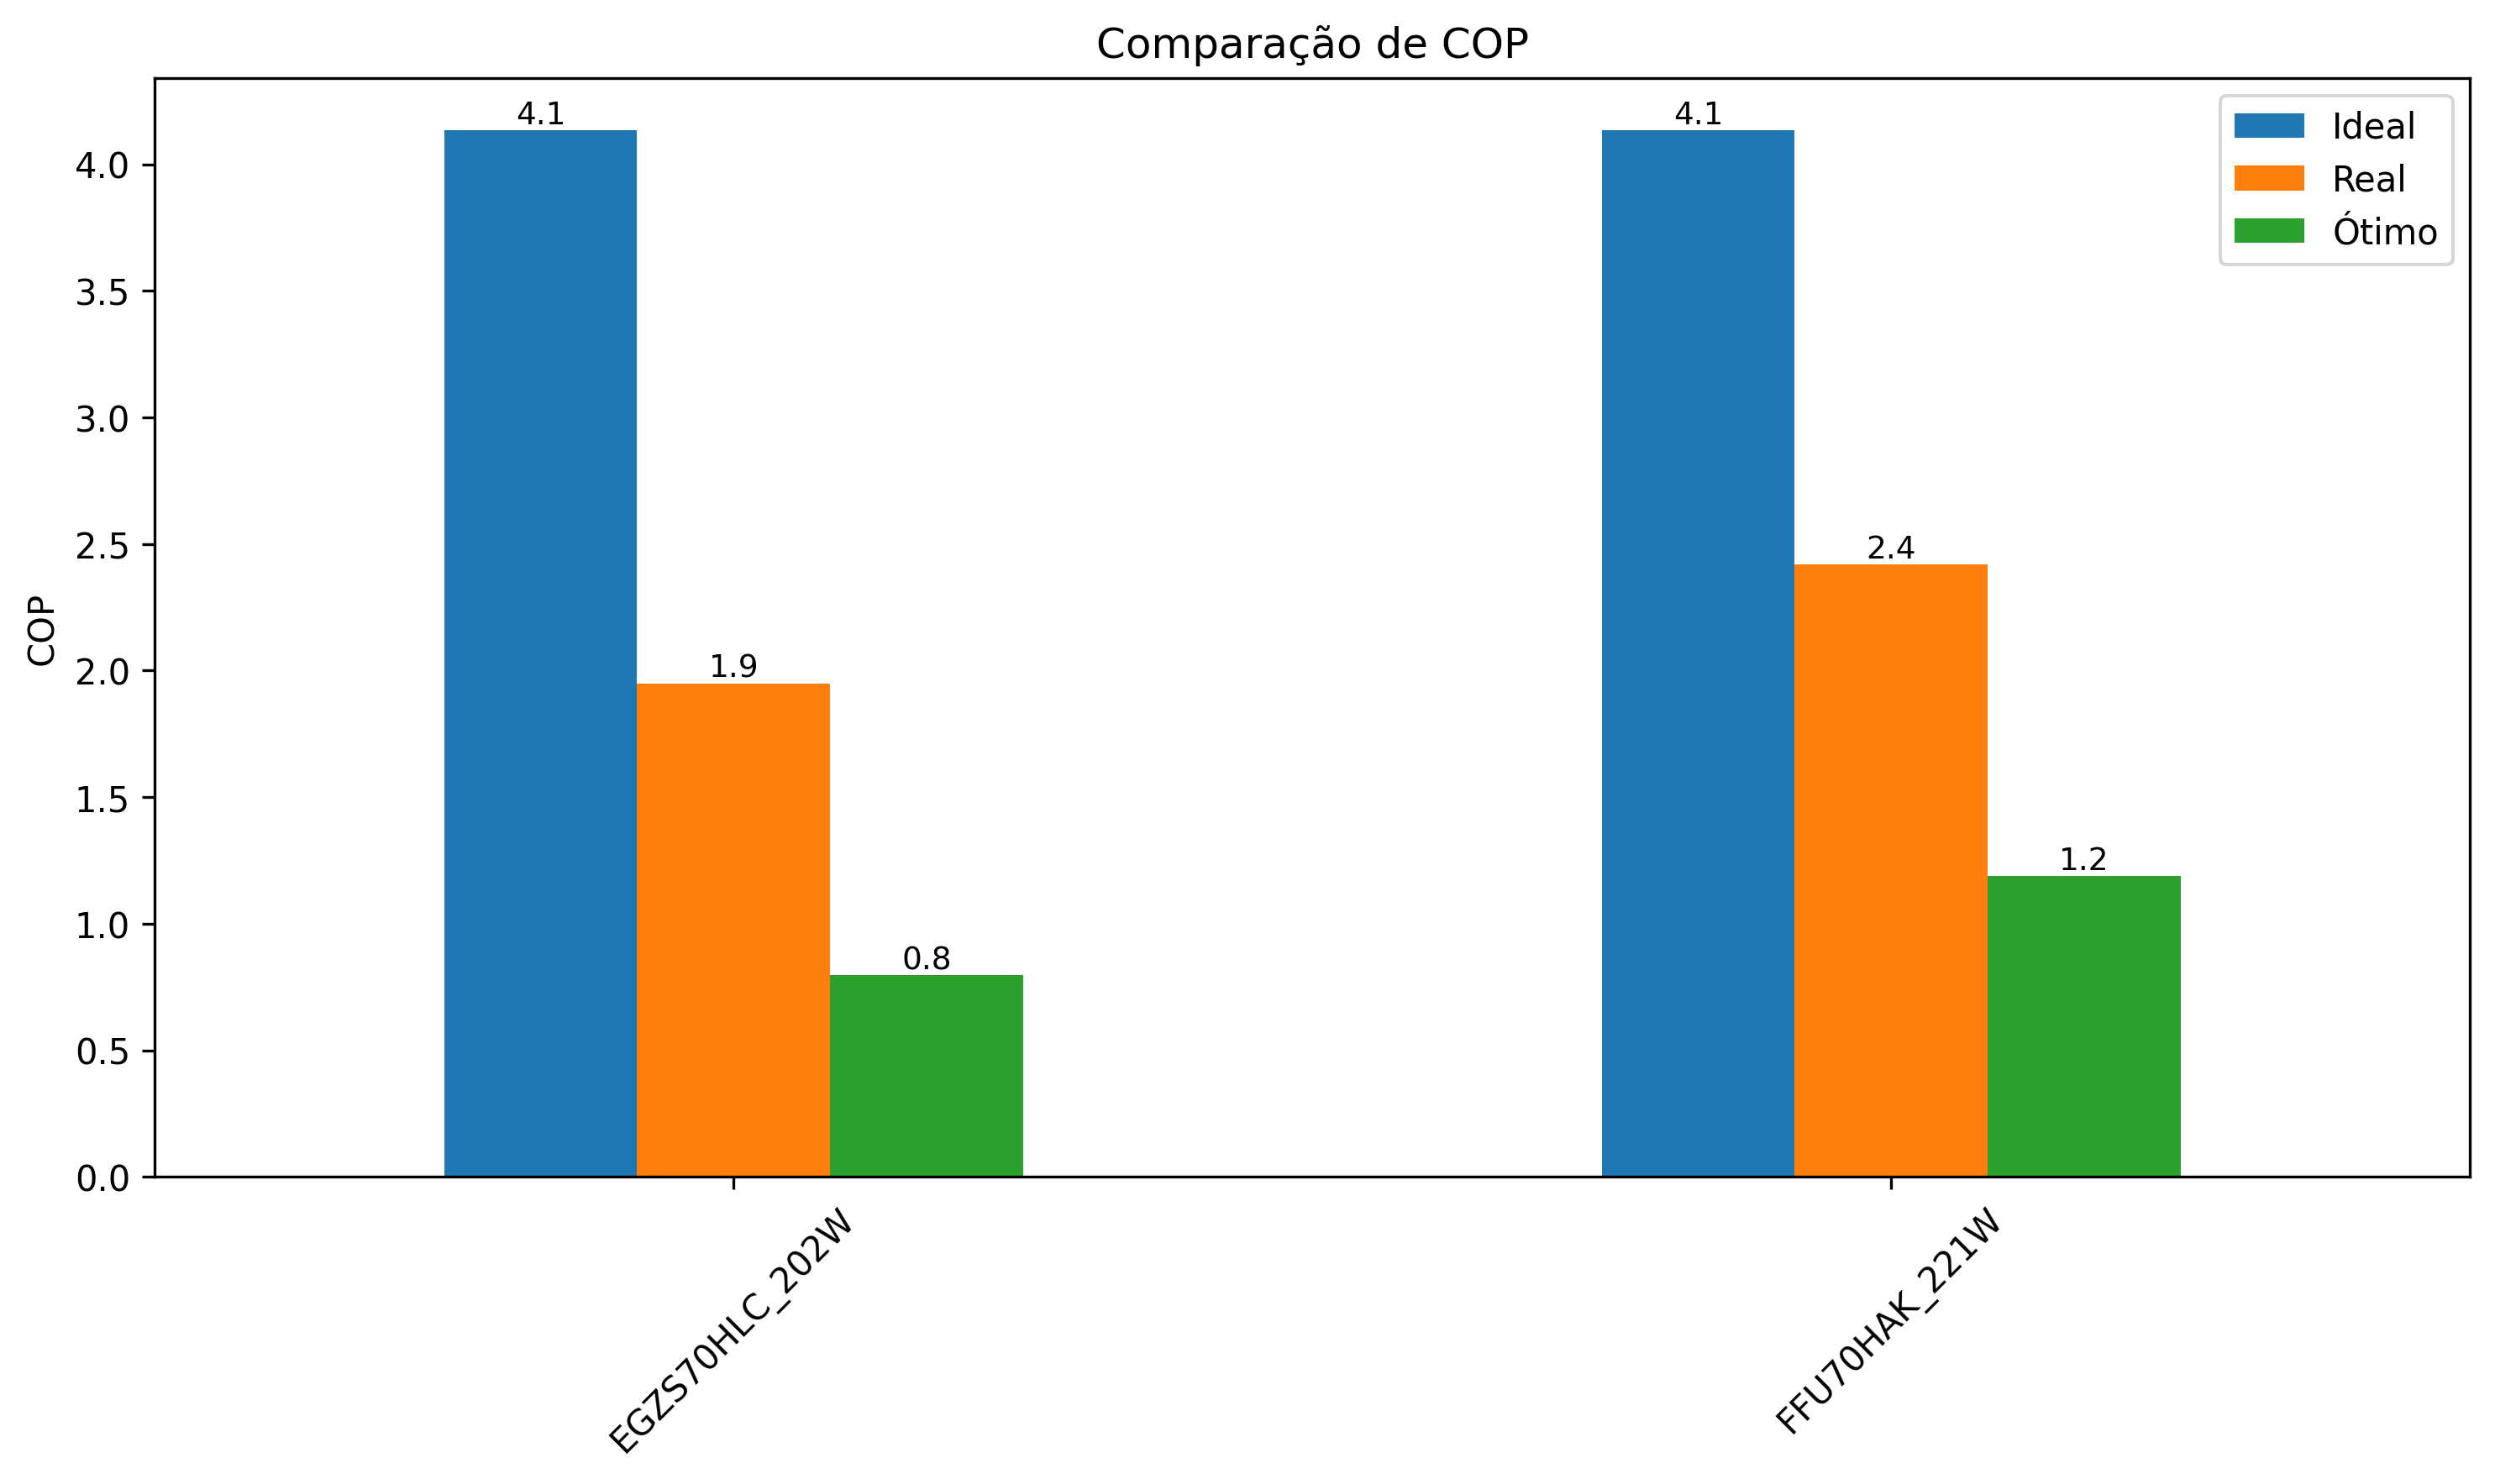
\includegraphics[width=0.8\linewidth]{Imagens/Desenvolvimento/barras_COP.png}
    \caption{Compração do COP.}
    \label{fig:barras COP}
\end{figure}

\begin{figure}[ht]
    \centering
    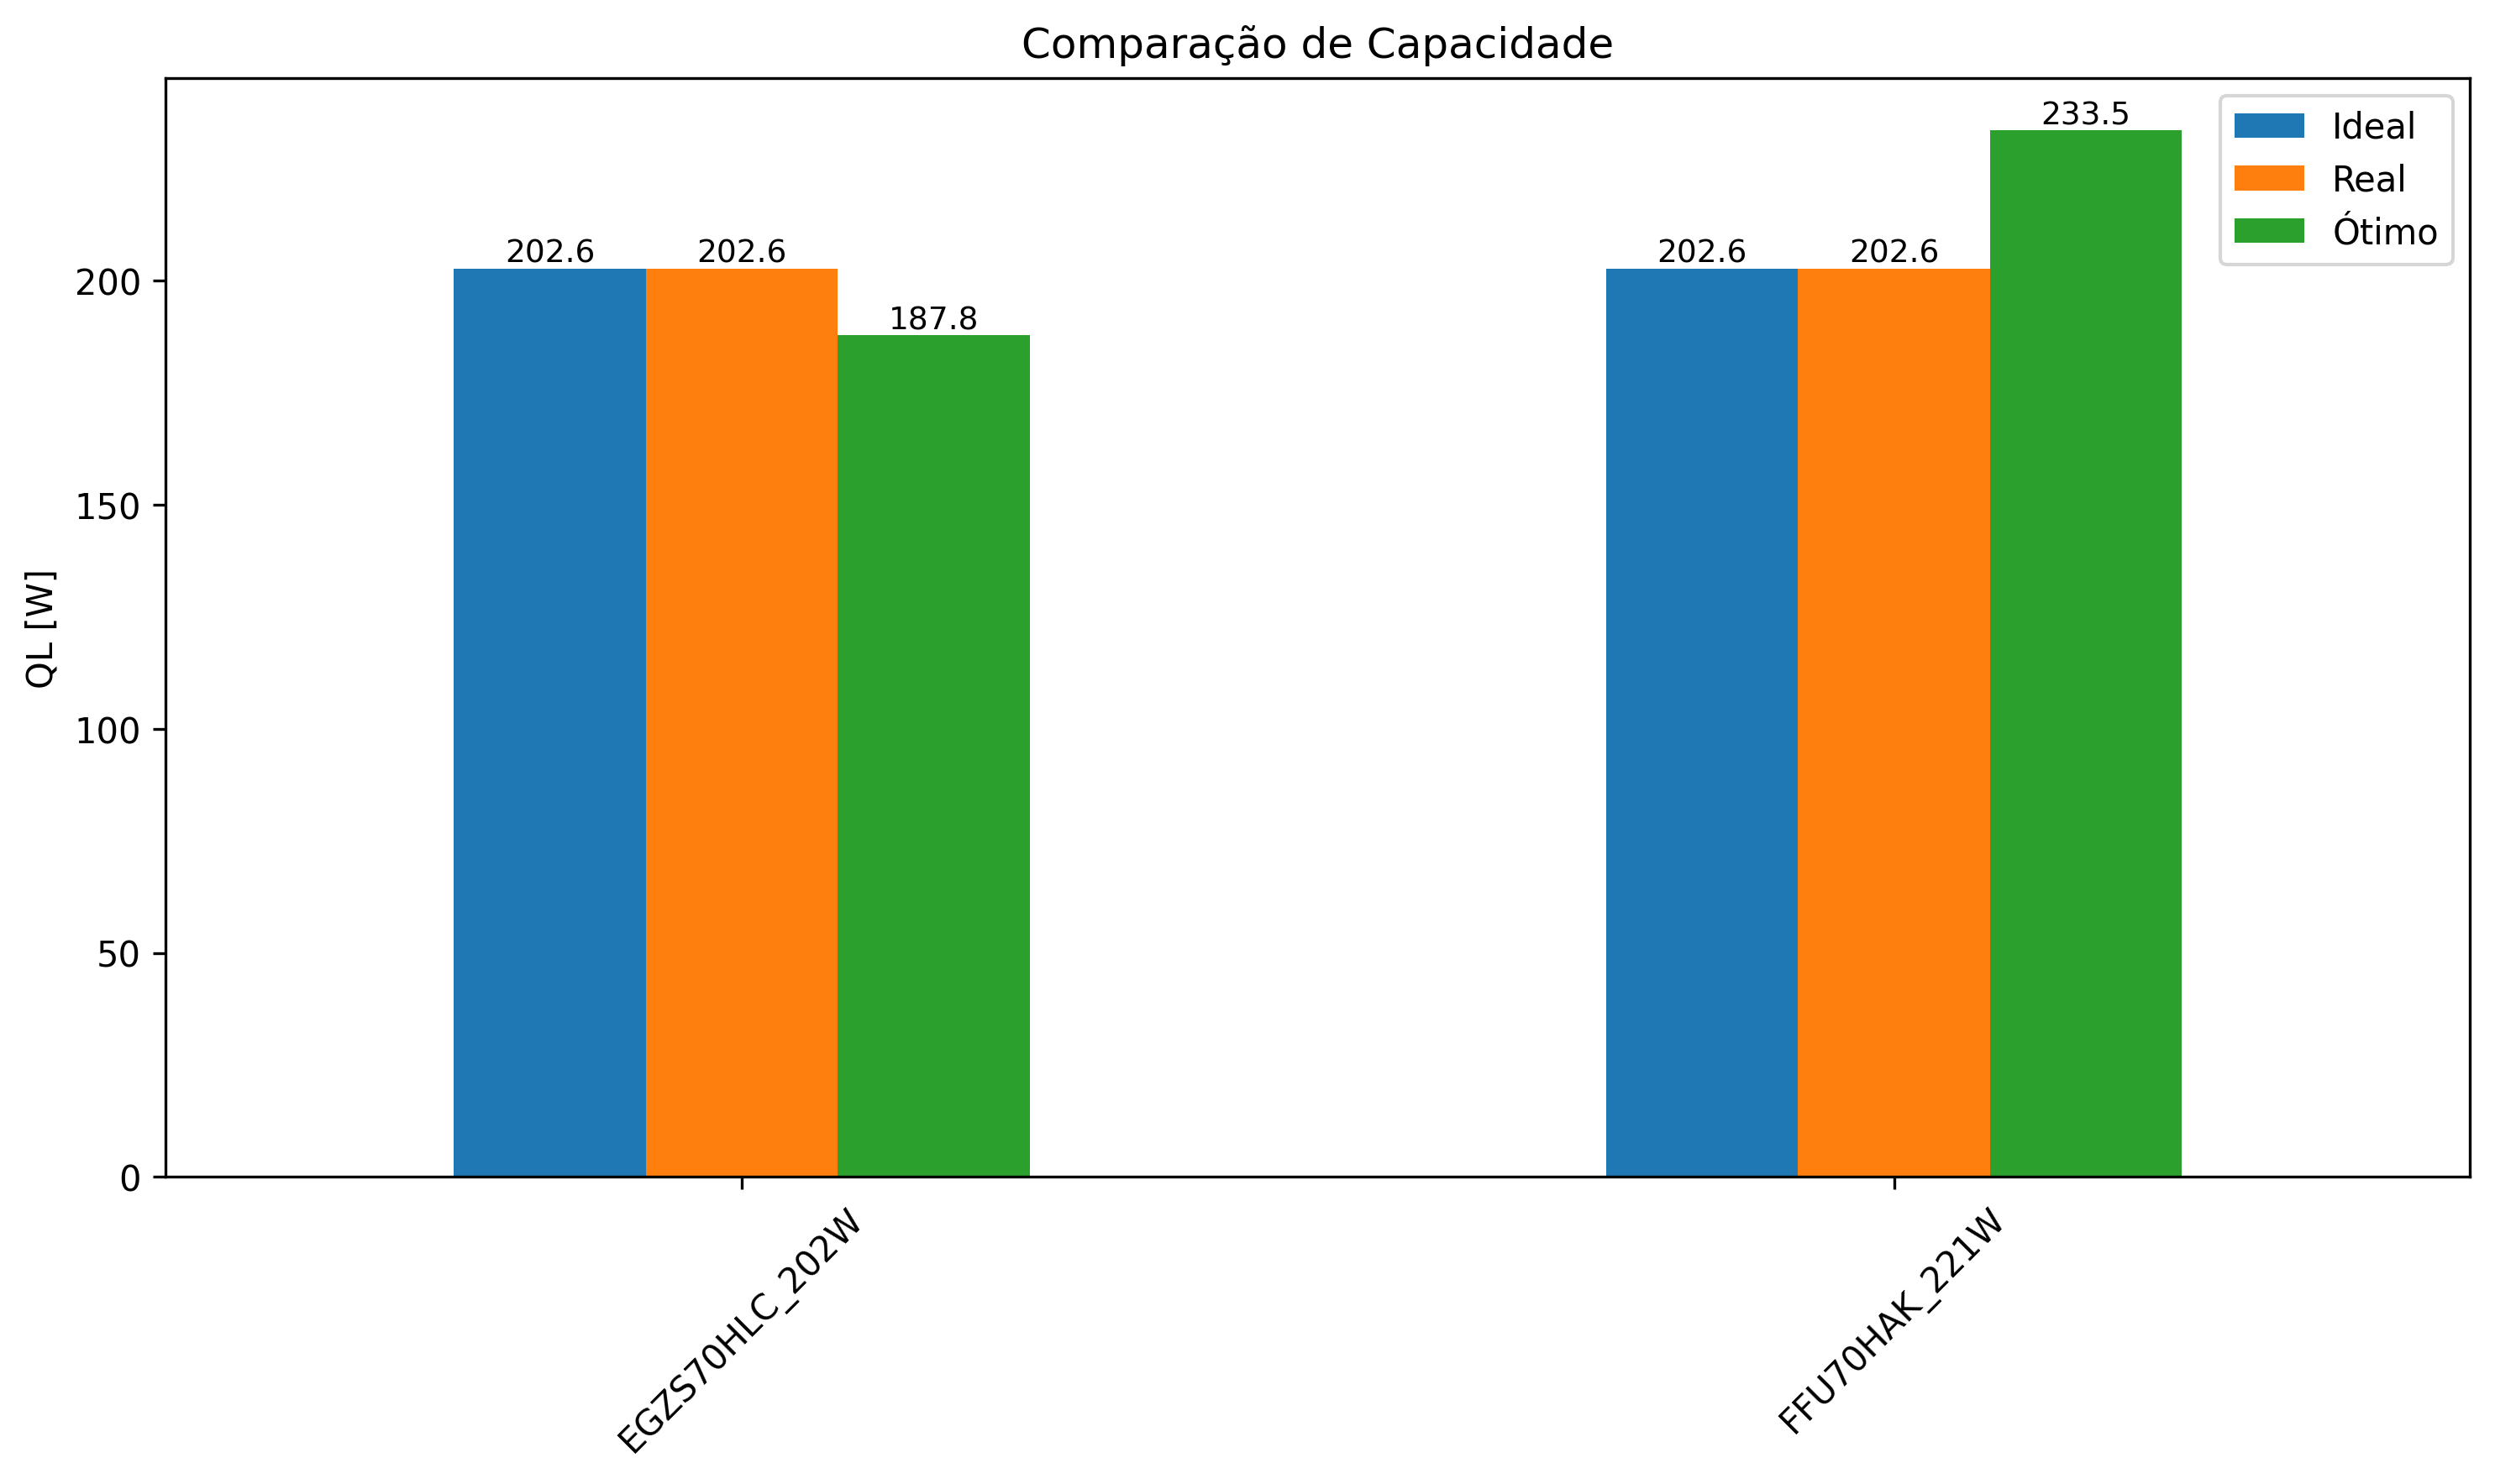
\includegraphics[width=0.8\linewidth]{Imagens/Desenvolvimento/barras_QL.png}
    \caption{Compração do $Q_L$.}
    \label{fig:barras Ql}
\end{figure}



Os resultados obtidos e mostrados nas Figuras \ref{fig:barras fluxo massa} a \ref{fig:barras Ql} demonstram a fidelidade do modelo computacional calculado com a base teórica, com  cada propriedade apresentando um comportamento esperado em cada situação.

    \begin{itemize}
        \item $\dot{m}$ : O ciclo ideal apresentou o menor valor para o fluxo mássico, enquanto os ciclos reais e ótimos aparecem com valores ligeiramente maiores, isso acontece pela necessidade de uma maior retirada de calor no sistema.
        \item COP : A máxima eficiência possível é determinada pelo ciclo de Carnot de refrigeração. A discrepância entre esse valor teórico e o desempenho no sistema real indica o quanto ele se afasta do ideal.
    \end{itemize}

